\chapter{Zadanie 3.}
Znormalizowana odpowied� skokowa(dla skoku jednostkowego) toru wej�cie-wyj�cie widoczna jest na rysunku ~\ref{odp_skok_u_z3}, natomiast toru zak��cenie-wyj�cie na rysunku ~\ref{odp_skok_z_z3}. Por�wnanie obu odpowiedzi wida� na rysunku ~\ref{odp_skok_obie_z3}. Zostan� one wykorzystane do wyznaczenia parametr�w algorytmu DMC. W szczeg�lno�ci odpowied� skokowa toru zak��cenie-wyj�cie zostanie wykorzystana w algorytmie, uwzgl�dniaj�cym zak��cenia, kt�ry powinien by� bardziej niezawodny ni� klasyczny algorytm.

\begin{figure}[b]
\centering
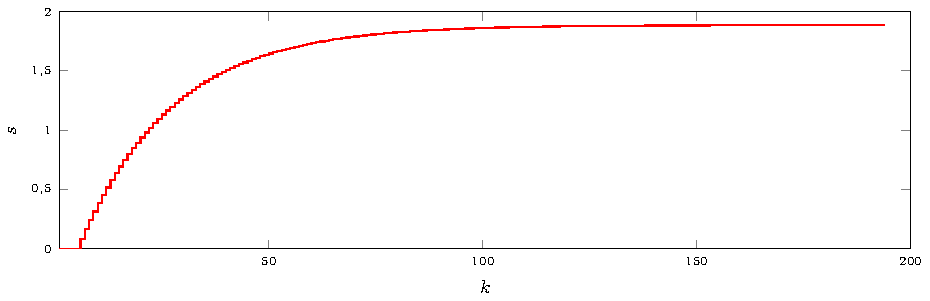
\includegraphics[scale=1]{../wykresy_pdf/odp_skok_jedn_ster.pdf}
\caption {Odpowied� skokowa toru wej�cie-wyj�cie}
\label{odp_skok_u_z3}
\end{figure}

\begin{figure}[b]
\centering
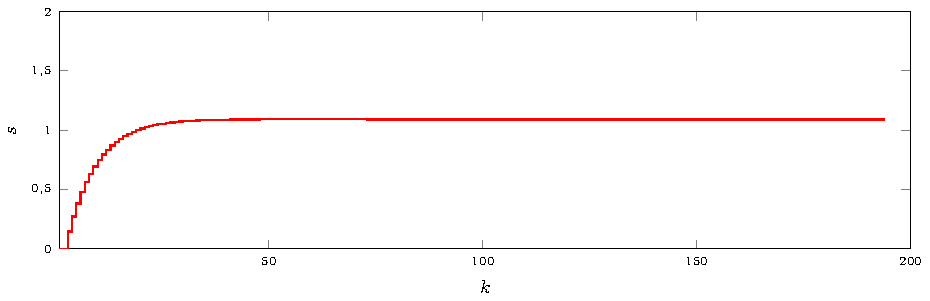
\includegraphics[scale=1]{../wykresy_pdf/odp_skok_jedn_zakl.pdf}
\caption {Odpowied� skokowa toru zak��cenie-wyj�cie}
\label{odp_skok_z_z3}
\end{figure}

\begin{figure}[b]
\centering
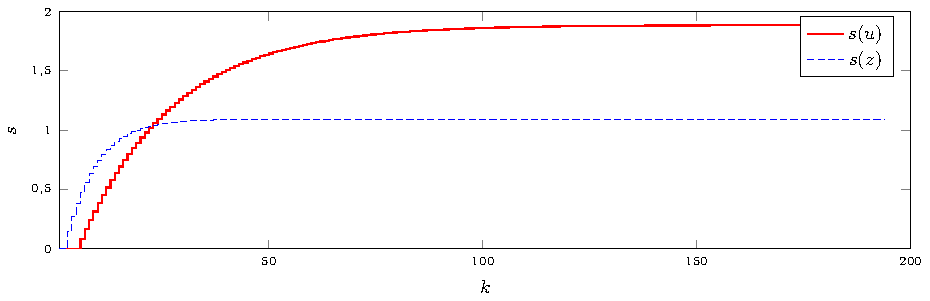
\includegraphics[scale=1]{../wykresy_pdf/odp_skok_jedn_oba.pdf}
\caption {Por�wnanie obu odpowiedzi}
\label{odp_skok_obie_z3}
\end{figure}